\section{Apprentissage artificiel}

\comment{}{Présentation plus générale s'inspirant de http://fr.wikipedia.org/wiki/Apprentissage_supervis\%C3\%A9. Note qu'il existe aussi un apprentissage non-supervisé qu'on ignore ici.}

D'un point de vue informatique, un algorithme d'apprentissage peut être vu comme un objet doté de 2 types de paramètres:
\begin{itemize}
 \item des paramètres dépendant des données qu'on va estimer à partir de données d'apprentissage notés $\theta$
 \item des paramètres fixés à la création de l'objet appelés hyper-paramètres
\end{itemize}
Son utilisation se fait en 2 phases:
\begin{itemize}
 \item une phase d'apprentissage (voir~\autoref{fig:Apprentissage_Machine}) au cours de laquelle on va estimer les paramètres $\theta$ grâce à 2 jeux de données:
       une matrice $X_{train}$ qui représente les données et une matrice $y_{train}$ qui représente les résultats correspondant aux données.
       On cherche en général des paramètres qui permettent d'optimiser un certain critère, notés $\theta^{*}$.
       Cependant, l'algorithme ne fournit pas en général les paramètres optimaux mais une approximation notée $\hat{\theta}$.

 \item une fois l'apprentissage effectué, on peut utiliser l'algorithme pour prédire les labels $y_{pred}$ associés à de nouvelles données $X_{test}$ (voir~\autoref{fig:Apprentissage_Machine_Prediction}).
\end{itemize}

\begin{figure}[htpb]
	\centering
	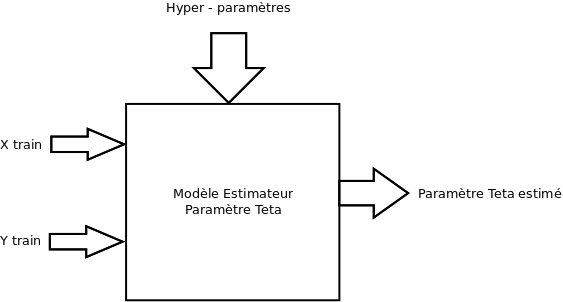
\includegraphics[scale = 0.25]{images/Diagramme1}
	\caption{Représentation de la phase d'apprentissage.}
	\label{fig:Apprentissage_Machine}
\end{figure}

% Ici, l'estimation du paramètre $\theta$ doit être tel que l'erreur estimé sur les prédictions soit le minimum possible. 
% Cette erreur est estimée selon un modèle de régression linéaire qui doit minimiser selon le paramètre $\theta$ par la méthode des moindres carrés, c'est-à-dire minimiser la formule suivante : 
% 
% \begin{equation}
% erreur = \sum_{i=1}^{n} (|y_{i} - \hat{y}_{i}|^{2})
% \end{equation}
% avec $y_{i}$ les vrais résultats et $\hat{y}_{i}$ les résultats estimés. 
% 
% Une fois que l'erreur a été estimé et que les $\theta$ ont été calculé, il est testé sur un échantillon test, suite à cela, la machine calcul une prédiction des résultats qu'on compare aux vrais résultats (voir~\autoref{fig:Apprentissage_Machine_Prediction}). 

\begin{figure}[htpb]
	\centering
	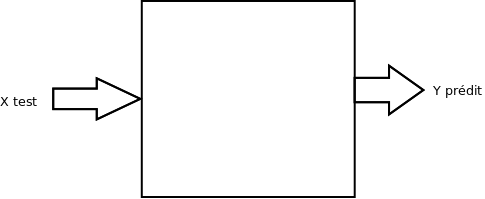
\includegraphics[scale = 0.25]{images/App_Mach_Prediction}
	\caption{Utilisation d'un algorithme pour la prédiction de nouvelles données.}
	\label{fig:Apprentissage_Machine_Prediction}
\end{figure}

\todo{expliquer l'apprentissage des k voxels}
